
% \documentclass[rascunho,xindy,acronym,symbols]{article}
% \usepackage[nolist,nohyperlinks]{acronym}

\documentclass[rascunho,xindy,acronym,symbols]{package/fei}

\usepackage[utf8]{inputenc}
%\usepackage[lmarging=3cm,tmargin=3cm,rmargin=2cm,bmargin=2cm]{geometry}
%\usepackage[onehalfspacing]{setspace}
%\usepackage[T1]{fontenc}
%\usepackage[brazil]{babel}

\usepackage{biblatex} %Imports biblatex package

\usepackage{url}
\usepackage{stix}
\usepackage{svg}
\usepackage{amsmath}
\usepackage{graphicx}
\usepackage{ulem}
\usepackage{pdfpages}


%\usepackage
%\usepackage[portugues,lined]{algorithm2e}
%\usepackage[breaklinks=true]{hyperref}
%\usepackage{breakcites}

% \usepackage{easyReview} % READICIONAR

%\newcommand\Tau{\mathcal{T}}
%%%% -- Configuracoes Iniciais
%%%%%%%%%%%%%%%%%%%%%%%%%%%%%%%%%%%%%%%%%%%%%%%%%%%%%%%%%%%%%%%%%%%%%%%%%%%%%%%%%%%%%%%%%%%%%%%%%%%%%%%%%

\author{Diogo F. de M. Santiago }
\title{Análise de MRI em Cardiomiopatia com o Apoio do Mecanismo de Atenção }
% \subtitulo{subtítulo}

%\cidade{Cidade}
%\instituicao{Instituição de Ensino}

%%%% -- Entradas Listas de Abreviaturas e Simbolos
%%%%%%%%%%%%%%%%%%%%%%%%%%%%%%%%%%%%%%%%%%%%%%%%%%%%%%%%%%%%%%%%%%%%%%%%%%%%%%%%%%%%%%%%%%%%%%%%%%%%%%%%%

%
\newacronym[]{SB}{SB}{\textit{size bunda}}
\newacronym[]{5G}{5G}{\textit{Fifth Generation Mobile Networks - Redes Móveis de Quinta Geração}}
 

\usepackage{caption}
\usepackage{subcaption}
\usepackage{lipsum}  

%% -- Simbolos
\newglossaryentry{A}{type=symbols,name={\ensuremath{A}},sort=a,description={exchanger total heat transfer area, $m^2$}}
\newglossaryentry{G}{type=symbols,name={\ensuremath{G}},sort=g,description={exchanger flow-stream mass velocity, $kg/(s m^2)$}}
\newglossaryentry{f}{type=symbols,name={\ensuremath{j}},sort=j,description={friction factor, dimensionless}}
\newglossaryentry{deltap}{type=symbols,name={\ensuremath{\Delta P}},sort=p,description={pressure drop, $Pa$}}
\newglossaryentry{nu}{type=symbols,name={\ensuremath{\nu}},sort=b,description={specific volume, $m^3/kg$}}
\newglossaryentry{beta}{type=symbols,name={\ensuremath{\beta}},sort=b,description={ratio of free-flow area $A_{ff}$ and frontal area $A_{fr}$ of one side of exchanger, dimensionless}}
\newglossaryentry{fr}{type=symbols,name={\ensuremath{fr}},sort=fr,description={frontal}}
\newglossaryentry{in}{type=symbols,name={\ensuremath{i}},sort=in,description={inlet}}
\newglossaryentry{out}{type=symbols,name={\ensuremath{o}},sort=out,description={outlet}}
%%%%%%%%%%%%%%%%%%%%%%%%%%%%%%%%%%%%%%%%%%%%%%%%%%%%%%%%%%%%%%%%%%%%%%%%%%%%%%%%%%%%%%%%%%%%%%%%%%%%%%%

\addbibresource{refs.bib}

\makeglossaries
\makeindex

\begin{document}

\maketitle
\begin{folhaderosto}
Proposta de Mestrado apresentada ao Centro Universitário FEI, como parte dos requisitos necessários para obtenção do título de Mestre em Engenharia Elétrica. Orientado pela Profa. Dra. Leila Cristina C. Bergamasco.
\end{folhaderosto}

 
% \fichacatalografica
% \folhadeaprovacao

% \dedicatoria{A quem eu quero dedicar o texto.}

% \include{agradecimentos}



% \epigrafe{A good scientist is a person with original ideas.
% A good engineer is a person who makes a design that works with as few original ideas as possible.
% There are no prima donnas in engineering.}{Freeman Dyson 
% \nocite{dyson_disturbing_1979}
% }

\begin{resumo}
% \lipsum[1-2]
Este trabalho consiste em unificar abordagens contemporâneas na avaliação da cardiomiopatia. Como apoio da análise radiômica, a qual extrai-se informações das características estatísticas e de textura de uma imagem médica e de \textit{features} oriundas de uma rede neural clássica para visão computacional, a \textit{ResNet50}, foi possível obter resultados promissores. Os resultados certificam que a união de informações de diversos âmbitos, a cerca de um dado paciente, quando aliadas, podem culminar em resultados mais interessados comparados quando avaliados os dados de forma isolada. O presente trabalho visa, usar as abordagens citadas, baseado em literaturas prévias, efetuando uma aplicação inédita para o teste de cardiomiopatia, adaptando e propondo uma arquitetura mais robusta de forma obter bons resultados.

\palavraschave{Radiomics, Mecanismo de Atenção, Transformers, Cardiomiopatia}
 
\end{resumo}
\begin{abstract}

\lipsum[2-4]

    
    
    \keywords{x,y,z}
\end{abstract}
% 
\newacronym[]{SB}{SB}{\textit{size bunda}}
\newacronym[]{5G}{5G}{\textit{Fifth Generation Mobile Networks - Redes Móveis de Quinta Geração}}
 



\listoffigures
%\listoftables
%\listofalgorithms
%\printacronyms
% \printglossaries

\tableofcontents

\chapter{Introdução}
\label{chap:intro}

A tecnologia \gls{SB} tem \gls{SB} \gls{5G} \gls{5G} perpetrado cada vez mais diversas áreas do saber, trazendo diversos benefícios e praticidades a vida contemporânea. Destas diferentes áreas, uma das que mais se beneficiaram com a tecnologia e a inovação foi a área médica. Desde meados dos anos 2000, a quantidade de dados disponível vêm crescendo exponencialmente se alcançando uma projeção de centenas de milhares de \textit{exabytes}(EB) para os anos de 2020 em diante \cite{gantzDIGITALUNIVERSE2020}.

Dada a enorme quantidade de dados gerados, a medicina tem se apoiado na utilização de dados clínicos textuais e principalmente imagens médicas, para a composição de seus diagnósticos. A análise de imagens médicas radiômicas é uma área em crescimento na medicina que se concentra na extração e análise de informações quantitativas e qualitativas destas imagens médicas, como tomografias computadorizadas (TC), ressonâncias magnéticas (RM) e imagens de ultrassom. Tanto a TC quanto a RM são exemplos de exames que podem gerar objetos tridimensionais (3D) de estruturas específicas do corpo humano a partir de dezenas de fatias \cite{book:1355375}. No entanto, apesar do progresso das técnicas de imagem cardíaca, o coração permanece sendo um órgão desafiador para se estudar. A inteligência artificial (IA) emergiu como uma das principais inovações no campo da imagem diagnóstica, com um impacto dramático na ressonância magnética cardiovascular (RMC). A inteligência artificial (IA) estará cada vez mais presente no mundo médico, com forte potencial para maior eficiência e precisão diagnóstica \cite{argentieroApplicationsArtificialIntelligence2022}.

A IA, composta por redes neurais profundas, também chamado de \textit{deep learning} (DL) dentro do espectro da visão computacional, podem ser utilizadas como classificadores, detectores de objetos, segmentadores, etc. Estas redes, com suas múltiplas camadas profundas, geram \textit{features} discriminantes após otimizadas a cerca de um conjunto de dados. Outro modelo de rede que vem tendo um uso cada vez maior e se encontra em diversas arquiteturas consagradas atuais, são as redes \textit{transformers}. As redes \textit{transformers} ficaram populares por serem comumente usadas em redes generativas auto-regressivas para geração sintética de texto, também conhecidas como \textit{large language models} (LLM), tenso seu exemplo mais conhecido no \textit{ChatGPT}. Os \textit{transformers} são arquiteturas que possuem como ponto forte principalmente sua capacidade de paralelismo e seu mecanismo de \textit{self-attention} que permite que o modelo se concentre nas partes relevantes dos dados de entrada, aprimorando a compreensão do contexto e das relações dentro dos dados.

Outra técnica também muito utilizada na análise de imagens médicas é a análise de textura (AT) que vem sendo usada por várias décadas em diversos domínios da medicina. Em oncologia, a AT de imagens de tomografia computadorizada mostrou correlação com a biologia tumoral subjacente ao diferenciar características histológicas diferentes e mutações genéticas específicas. Em malignidades estabelecidas, a AT se relaciona com a histologia do tumor em muitos tumores sólidos comuns (pulmão, colorretal, esofágico, mama), ela se correlaciona com mutações genéticas específicas e pode acompanhar respostas terapêuticas. Fora da oncologia, mudanças não malignas em órgãos podem ser detectadas (por exemplo, cirrose hepática e pneumonite intersticial usual). Dentro da imagem cardíaca, a AT aplicada à ressonância magnética cardiovascular tem sido usada para avaliar o risco de arritmia pós-infarto do miocárdio, o uso da RMC em imagens sem contraste e com realce tardio de gadolínio em pacientes com cardiomiopatia hipertrófica (CH) para prever o resultado é uma área de interesse particular atualmente \cite{schofieldTextureAnalysisCardiovascular2019a}.

A área da análise radiômica consiste no processo de obter dados qualitativos destas imagens de radiografias combinadas, por vezes, a extração de textura destas mesmas imagens. A análise radiômica pode até ser usada para avaliar a resposta ao tratamento ou para transmitir certas características prognósticas. Dentre as doenças do coração, a cardiomiopatia hipertrófica (CH) é desenvolvida prioritariamente em jovens e pessoas de meia idade, sendo a mais comum das cardiomiopatias . Mesmo que a CH se apresente de forma assintomática em parte dos casos, esta pode culminar em morte súbita cardíaca, insuficiência cardíaca, acidente vascular cerebral e arritmia \cite{kwonComparisonMortalityCause2022}. A análise radiômica auxilia com diagnóstico prévio afim de compreender e atuar em caso de CH que demonstrem risco ao paciente.

% Algumas de suas características são: extração de características, quantificação e padronização, possibilidade de correlação com dados clínicos. As aplicações da análise radiômica consiste em diversas aplicações clínicas, incluindo diagnóstico auxiliado por computador, predição de resposta ao tratamento, estratificação de pacientes, identificação de biomarcadores e personalização de tratamentos.

Este trabalho tem como ideia principal unir tanto as \textit{features} radiômicas quanto as \textit{features} profundas, assim chamadas por serem extraídas de modelo de IA, para com um modelo de arquitetura proposto, que se utiliza de \textit{self-attention}, analisar e prever a cardiomiopatia hipertrófica. O uso destas duas abordagens aliadas na extração de características a cerca da doença, tem o potencial de obter resultados melhores resultados preditivos se comparados as técnicas isoladas. Neste trabalho é proposta a estratégia de fusão de múltiplas fontes, que combina as \textit{features} manuais extraídas da análise de textura radiômica e as \textit{features} profundas, para melhorar a expressividade e a habilidade de generalização do modelo.

\newpage

% \section{Motivação}

\section{Objetivo}

\subsection{Objetivos Específicos}

Como objetivo desta dissertação, espera-se obter os seguintes resultados:

\begin{enumerate}

\item Execução de modelo, que utilizas as \textit{features} radiômicas e
\textit{deep features} e coleta de resultados em conjunto de dados públicos.

\item Avaliação dos resultados iniciais

\item Proposta de novas abordagens tanto no pré-processamento quanto na arquitetura, mediante coleta dos resultados.

\item Iteração e análise dos resultados obtidos, sua documentação e comparação.
\end{enumerate}


\section{Estrutura do trabalho}

\textcolor{lightgray}{
Esta proposta de dissertação está organizada em seis capítulos, a saber:
O \textbf{Capítulo \ref{chap:intro}} apresenta a introdução, motivação, objetivo e contribuições desejadas. O \textbf{Capítulo \ref{chap:fundamentacao_teorica}} fará um aprofundamento teórico no tema de pesquisa estudando as principais técnicas que serão utilizadas para o desenvolvimento do experimento prático. No \textbf{Capítulo \ref{chap:trab_relacionados}} é estudado  os trabalhos recentes, não superior a cinco anos passados, de outros autores que estão relacionados com tema.  No \textbf{Capítulo \ref{chap:metodologia}} é apresentada uma proposta de metodologia  para a realização do experimento prático.\\ O \textbf{Capítulo \ref{chap:proposta}} é uma proposta experimental que contempla os materiais provisionados para a execução e o cronograma do presente projeto de pesquisa. No \textbf{Capítulo \ref{chap:resultados_discussao}}, são apresentados os resultados parciais da proposta experimental e também são discutidos e argumentados os resultados parciais. Finalmente, o \textbf{Capítulo \ref{chap:conclusao}} apresenta conclusão do presente projeto de pesquisa.
}

\chapter{Fundamentação Teórica}
\label{chap:fundamentacao_teorica}

A proposta deste trabalho visa unificar informações das \textit{features} radiômicas e \textit{features} profundas oriundas de uma rede neural convolucional e, por conseguinte, propor uma arquitetura de \textit{self-attention} para identificar características discriminantes afim de obter resultados relevantes na classificação de cardiomiopatia hipertrófica. Os fundamentados os seguintes conceitos: análise radiômica, extração de \textit{features} profundas e redes \textit{transformers}.

%--------------------------------------------------------
\section{Ressonância Magnética em Cardiomiopatia}

A ressonância magnética (RM) está se tornando o principal método de imagem para avaliar a fisiologia e a função na doença cardíaca congênita. A RM possui funções que normalmente são obtidas por ecocardiografia, tendo como exemplo a velocidade média em um vaso, mas também apresenta características muito especiais como calcular a velocidade em um voxel de um milímetro em qualquer lugar no espaço tridimensional do vaso.
Usando a tecnologia atual de RM, os investigadores podem obter percepções únicas sobre a função ventricular, por exemplo, deformação ventricular regional in vivo e movimento da parede e mecânica dos fluidos, por exemplo, visualização in vivo de perfis de velocidade além de aumentar a precisão de medidas padrão aceitas pela fisiologia ou função ventricular, por exemplo, débito cardíaco, volumes ventriculares e massa. Devido ao rápido avanço da tecnologia, muitas técnicas de RM são experimentais ou ainda estão em fase de desenvolvimento clínico; no entanto, há muitas técnicas que são clinicamente úteis, por exemplo, medição do volume ventricular em pacientes com tamanho ventricular esquerdo limítrofe. Como muitas das técnicas experimentais atuais serão, sem dúvida, empregadas na prática clínica no futuro, os médicos devem estar cientes de todo o espectro de capacidades da RM \cite{fogelAssessmentCardiacFunction2000}.

Em muitos cenários clínicos, as limitações técnicas da ecocardiografia e a expressão fenotípica heterogênea tornaram tal avaliação difícil, e a RM cardíaca emergiu como uma modalidade de imagem complementar útil para complementar a ecocardiografia transtorácica de rotina. A RM cardíaca é única em sua alta resolução espacial e temporal com excelente contraste entre o pool sanguíneo e o miocárdio, sem limitação de janela de imagem ou plano de imagem.
A heterogeneidade fenotípica da miocardiopatia hipertrófica é bem reconhecida pela dificuldade em sua identificação. Isto se complica ainda mais pois nem todos os pacientes com hipertrofia ventricular esquerda têm CMH, enquanto uma fisiopatologia semelhante à CMH com obstrução dinâmica do trato de saída do ventrículo esquerdo pode ser observada sem hipertrofia do ventrículo esquerdo, em um subgrupo de pacientes com anormalidades na válvula mitral e/ou no músculo papilar.

A CMH é uma doença heterogênea com expressão morfológica complexa que requer uma caracterização precisa da doença para um planejamento terapêutico ótimo e estratificação de risco. A RM cardíaca emergiu como um complemento útil para esses propósitos. Com a incorporação crescente de imagem multimodal na avaliação clínica da CMH, nosso entendimento sobre a importância de diferenças morfológicas sutis continuará a crescer, e pesquisas adicionais definirão novos marcadores prognósticos e melhorarão as estratégias de tratamento atuais\cite{toCardiacMagneticResonance2011c}.


%Diferentemente de outras áreas que utilizam e geram majoritariamente dados textuais, a Medicina também faz uso massivo de imagens para composição de seus diagnósticos. Independentemente do propósito da imagem, nos últimos anos esses equipamentos também evoluíram e se tornaram mais precisos, proporcionando um volume maior de dados e imagens, que exigem uma maior capacidade de armazenamento (ISSA; BYERS; DAKSHANAMURTHY, 2014).

%Algumas modalidades médicas como a Ressonância Magnética Cardíaca (RMC) e a Tomografia Computadorizada (TC) são exemplos de exames que podem gerar objetos tridimensionais (3D) de estruturas específicas do corpo humano a partir de dezenas de fatias (BANKMAN; MORCOVESCU, 2002). Um outro aspecto que também desafia a comunidade médica é a fadiga visual, percebida quando o especialista realiza a análise contínua de muitas imagens.


% Expostos esses fatores, torna-se relevante o desenvolvimento de métodos inteligentes para armazenamento e recuperação dessas imagens médicas que são geradas diariamente. Nesse sentindo, os sistemas de Diagnóstico Auxiliado por Computador (Computer-Aided Diagnosis - CAD) têm o propósito de apoiar especialistas médicos em seus diagnósticos, uma vez que o tempo demandado para analisar essas imagens tem se tornado cada vez maior (DATTA et al., 2008).

%--------------------------------------------------------
\section{Análise Radiômica}

A análise radiômica é um campo de pesquisa em rápida evolução, preocupado com a extração de informações quantitativas, incluindo padrões complexos que são difíceis de reconhecer ou quantificar pelo olho humano dentro de imagens médicas, características estas chamadas  de\textit{features} radiômicas. As \textit{features} radiômicas podem capturar características de tecidos e lesões, como forma e heterogeneidade, e podem, sozinhas ou em combinação com dados demográficos, histológicos, genômicos ou proteômicos, ser usadas para a resolução de problemas clínicos. O objetivo desta seção é fornecer uma introdução ao campo, cobrindo o fluxo de trabalho básico da análise radiômica: cálculo e seleção de características, redução de dimensionalidade e processamento de dados \cite{mayerhoeferIntroductionRadiomics2020}.

Embora \textit{features} radiômica individuais podem se correlacionar com dados genômicos ou dados clínicos, o impacto da análise radiômica se torna mais relevante a medida que mais informações são por ela extraídas. Tipicamente centenas de \textit{features}, uma fração das do total extraído, contribuem para identificação de uma doença específica e é processada usando técnicas de aprendizado de máquina.

As \textit{features} radiômicas podem ser subdivididas em estatísticas, incluindo as baseadas em histograma e textura; modelo; transformação; e forma. A extração pode ser dada em regiões de interesse de 2-dimensões (2D) e 3-dimensões (3D).

%--------------------------------------------------------
\subsection{\textit{Features} por Histograma}

Os descritores estatísticos mais simples são baseados no histograma global de níveis de cinza e incluem média de nível de cinza, máximo, mínimo, variância e percentis. Como essas características são baseadas em análises de pixel único ou voxel único (3D), elas são chamadas de características de primeira ordem. Algumas \textit{features} mais sofisticadas incluem assimetria e curtose que descrevem a forma da distribuição de intensidade dos dados: a assimetria reflete a assimetria da curva de distribuição dos dados para a esquerda (assimetria negativa, abaixo da média) ou direita (assimetria positiva, acima da média), enquanto a curtose reflete a caudalidade de uma distribuição de dados em relação a uma distribuição gaussiana devido a \textit{outliers}. Outras \textit{features} incluem histograma entrópico e uniformidade (também chamado de energia).

%--------------------------------------------------------
\subsection{\textit{Features} de Textura}

Uma abordagem simples para a descrição de textura radiômica é a análise do gradiente absoluto, que reflete o grau ou a abruptidade das flutuações de intensidade de nível de cinza em uma imagem. Para dois \textit{pixels} ou \textit{voxels} adjacentes, o gradiente é o máximo possível quando um for preto e o outro branco, enquanto se ambos os \textit{pixels} forem pretos (ou ambos forem brancos) o gradiente nessa localidade é zero. Similares as \textit{features} por histograma, as \textit{features} por gradiente incluem média, variância, assimetria e curtose (Fig. \ref{fig:fig001}).

\captionsetup{justification=centering}
\begin{figure}[htbp]
    \centering
    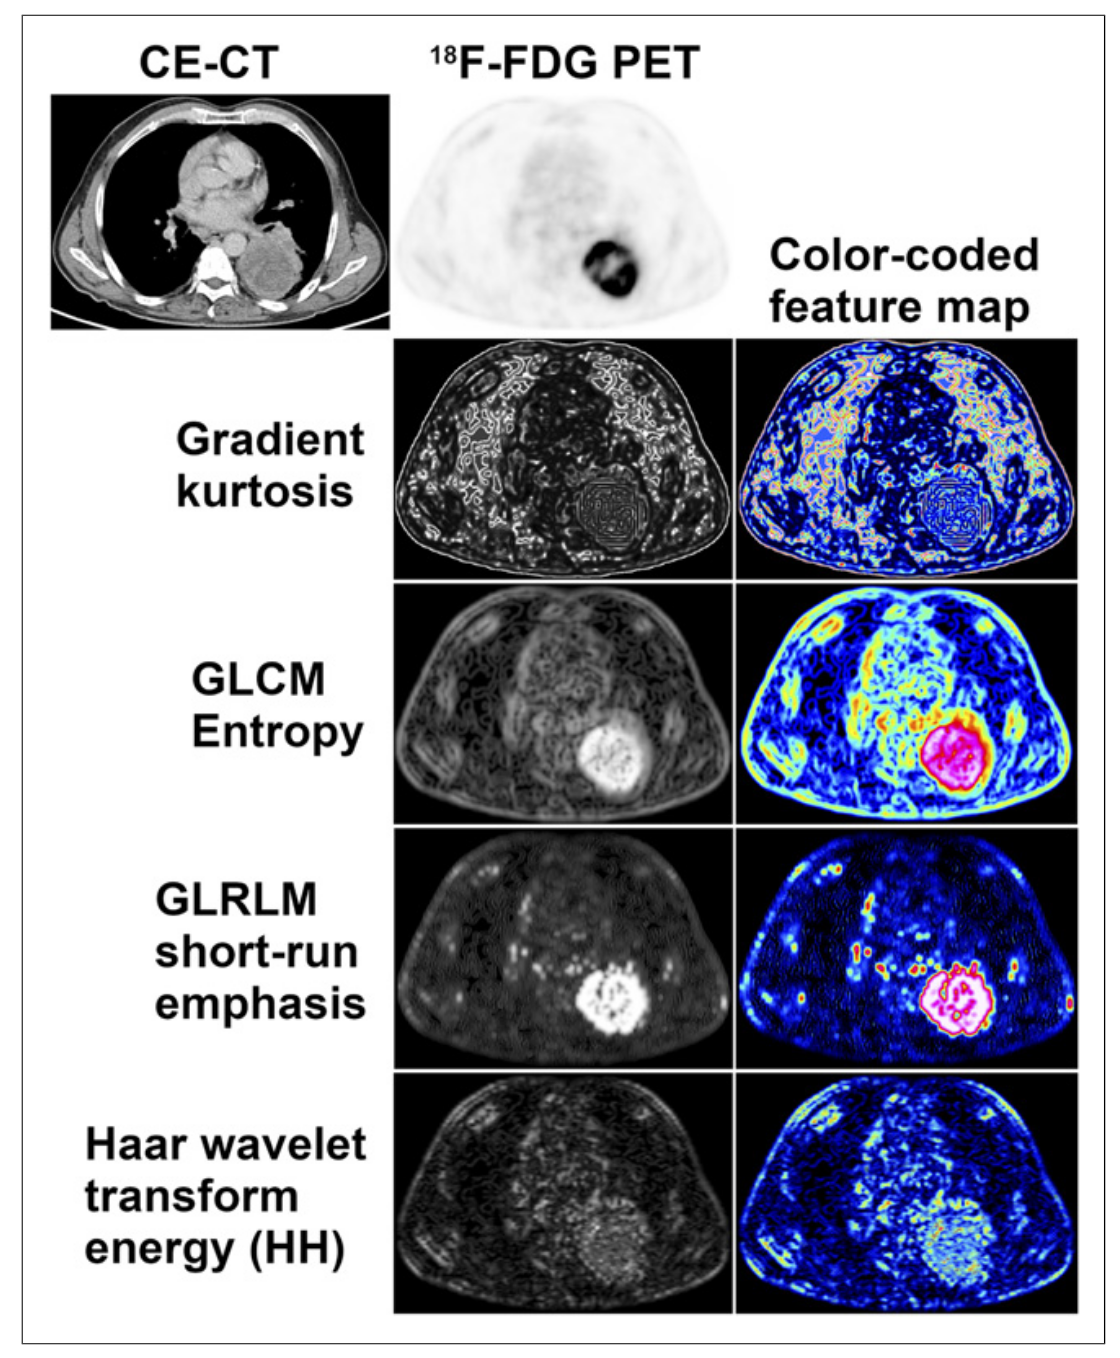
\includegraphics[width=0.6\textwidth]{figures/fig001.png}
    \caption{Exemplos de análise radiômica.}
    \label{fig:fig001}
\end{figure}

 \textit{GLCM}. A matriz de coocorrência de níveis de cinza, do termo \textit{Gray-Level Cooccurrence Matrix} (GLCM) é um histograma em níveis de cinza de segunda ordem. O GLCM captura relações espaciais entre pares de \textit{pixels} ou \textit{voxels} com níveis de níveis de cinza pré-definidos, em diferentes direções (horizontal, vertical ou diagonal para análise 2D, 13 direções para 3D) e com uma distância pré-definida entre os \textit{pixels} ou \textit{voxels} (Fig. \ref{fig:fig002}). As \textit{features} de GLCM incluem entropia (Fig. \ref{fig:fig002}), uma medida de  compostas por uma medida da inomogeneidade ou aleatoriedade dos níveis de cinza, momento angular de segunda ordem (também chamado de uniformidade ou energia), que reflete a homogeneidade ou ordem dos níveis de cinza e contraste, que enfatiza as diferenças nos níveis de cinza entre \textit{pixels} ou \textit{voxels} pertencentes a um par de \textit{pixel} ou \textit{voxel}.

 \textit{GLRLM}. A matriz de comprimento de corrida de níveis de cinza, do termo 
 \textit{Gray-Level Run-length Matrix} (GLRLM) fornece informações sobre a distribuição espacial das sequências de \textit{pixels} consecutivos com os mesmos níveis de cinza, em uma ou mais direções, em 2 ou 3 dimensões. As características da GLRLM incluem fração, que avalia a porcentagem de \textit{pixels} ou \textit{voxels} dentro da região de interesse que fazem parte das sequências e, portanto, reflete a granulosidade. 

\textit{GLSZM}. A matriz de zona do tamanho dos níveis de cinza, do termo \textit{Gray-Level Size Zone Matrix} (GLSZM) é baseada no mesmo princípio do GLRLM porém aqui, contagens do número de grupos (chamados zonas) de pixels ou voxels vizinhos interconectados com o mesmo nível de cinza formam a base para a matriz (Fig. \ref{fig:fig002}. Uma textura mais homogênea resultará em uma matriz mais ampla e plana. A GLSZM não é calculada para diferentes direções, mas pode ser calculada para diferentes distâncias de pixels ou voxels que definem a vizinhança. As \textit{features} da GLSZM podem ser calculadas em 2 dimensões (8 pixels vizinhos) ou 3 dimensões (26 voxels vizinhos) e, seguindo as definições da GLRLM, incluem fração (porcentagem de pixels ou voxels que fazem parte das zonas), ênfase em zonas grandes e pequenas, entre outras.

\begin{figure}[htbp]
    \centering
    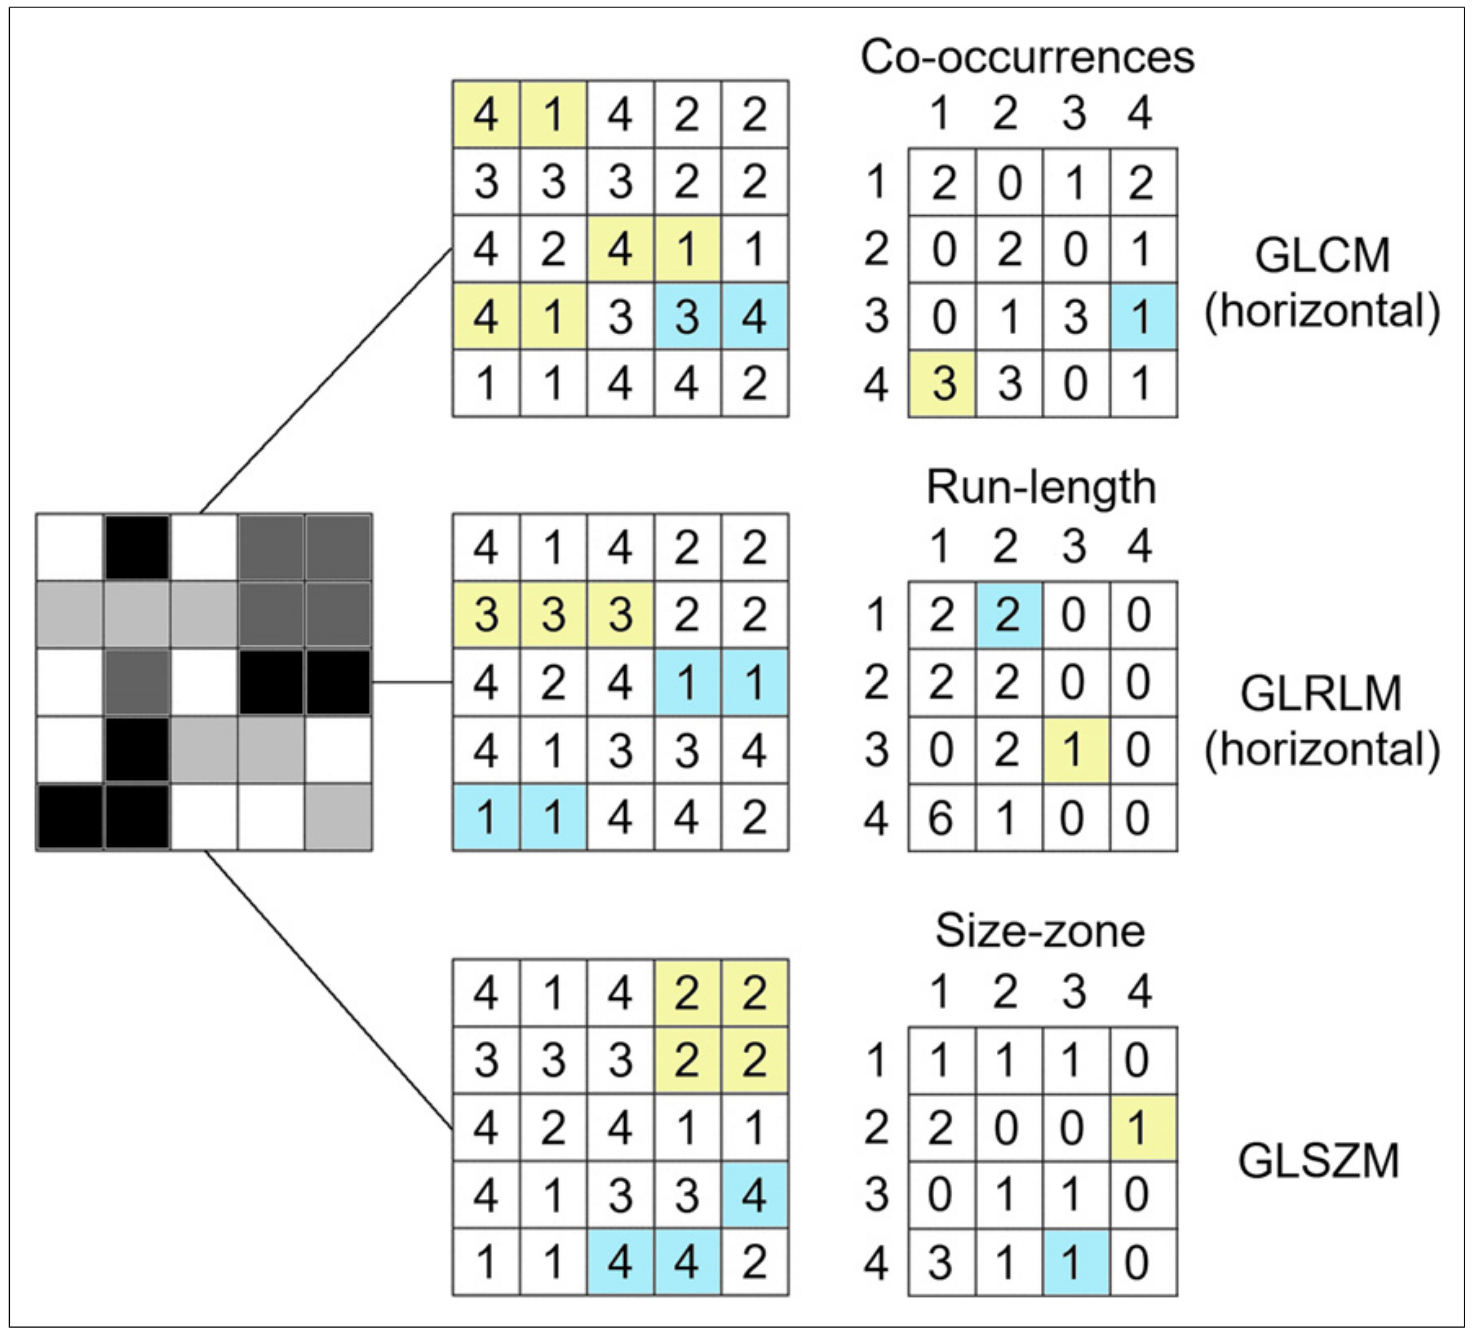
\includegraphics[width=0.6\textwidth]{figures/fig002.png}
    \caption{Exemplos de análise radiômica.}
    \label{fig:fig002}
\end{figure}

%--------------------------------------------------------
\subsection{\textit{Features} de Modelo}

As análises baseadas em modelos visam interpretar \textit{features} em níveis de cinza espaciais para caracterizar objetos ou formas. Um modelo parametrizado de geração de textura é calculado e ajustado à região de interesse (ROI), e seus parâmetros estimados são utilizados como \textit{features} radiômicas. O modelo autorregressivo é um exemplo de abordagem baseada em modelo e baseia-se na ideia de que o nível de cinza de um pixel é uma soma ponderada dos níveis de cinza de 4 pixels vizinhos. Além disso, $\sigma$, a qual carrega informações sobre a variância do erro de previsão mínimo, mede a regularidade da textura. A análise fractal também produz recursos que podem ser usados na análise radiômica, em particular a dimensão fractal, que reflete a taxa de adição de detalhe estrutural com o aumento da magnificação, escala ou resolução e, portanto, serve como uma medida de complexidade. A lacunaridade, um recurso que mede a falta de invariância rotacional ou translacional, reflete a inomogeneidade \cite{mayerhoeferIntroductionRadiomics2020}.

%--------------------------------------------------------
\subsection{\textit{Features} de Transformação}
Métodos Baseados em Transformadas, incluindo transformadas de \textit{Fourier}, \textit{Gabor} e de \textit{wavelets} de \textit{Haar}, analisam padrões de níveis de cinza em um espaço diferente. A transformada discreta de \textit{wavelet} de \textit{Haar}, por exemplo, analisa o conteúdo da frequência de uma imagem em diferentes escalas. A decomposição por \textit{wavelets} de uma imagem é possível aplicando um par de filtros espelhados em quadratura, um filtro de passa-alta e um de passa-baixa. Embora o filtro de passa-alta destaque as mudanças no nível de cinza e, assim, enfatize detalhes da imagem, o filtro de passa-baixa suaviza a imagem em termos de nível de cinza, removendo detalhes da imagem. Após a decomposição do sinal, um conjunto de canais de frequência orientados espacialmente está disponível, o qual é usado para descrever a variabilidade local da imagem. As energias dentro dos canais de frequência são então usadas como \textit{features}. A filtragem de passa-alta em ambas as direções (Fig. \ref{fig:fig001}) captura detalhes diagonais, a filtragem de passa-alta seguida por filtragem de passa-baixa captura bordas verticais, a filtragem de passa-baixa seguida por filtragem de passa-alta captura bordas horizontais, e a filtragem de passa-baixa em ambas as direções captura as frequências mais baixas, em diferentes escalas. Notavelmente, a transformação por \textit{wavelets} pode ser usada não apenas para a geração de \textit{features} radiômicas, mas também para segmentação de imagens ou como um passo de pré-processamento para análise de textura \cite{mayerhoeferIntroductionRadiomics2020}.

%--------------------------------------------------------
\section{Extração de Features Profundas}
Para extrair \textit{features} profundas das imagens de RM, foi empregada a arquitetura pré-treinada de uma rede \textit{ResNet50}. As redes \textit{ResNet50} ficaram muito conhecidas ao fim do ano de 2015 por vencer diversas competições em visão computacional, includindo 1º lugar na competição de classificação de imagens \textit{ILSVRC} 2015. As redes \textit{ResNet}, do termo \textit{Residual Networks}, inovaram na em sua época trazendo uma forma de treinar modelos de maior profundidade, chegando a mais de 100 camadas, com resultados superiores à outros modelos convolucionais competitivos, como o \textit{VGG19}, sem sofrer os sintomas comum a estas redes muito profundas que seriam o de \textit{overfitting} e a saturação/ausência dos gradientes em tempo de treino. Os autores da \textit{ResNet} sugeriram o uso de saltos de conexão entre as camadas da rede (Fig. \ref{fig:fig003}) afim de manter os gradientes relevantes e controlados entre uma camada e outra.  A \textit{ResNet50} é um modelo de rede neural convolucional profunda de 50 camadas que compreende muitos blocos residuais. Cada bloco contém módulos de convolução e uma conexão de salto que transfere a informação do bloco anterior para o próximo bloco. A conexão de salto ajuda a reter a informação semântica mais baixa aprendida nas camadas anteriores, que de outra forma se tornaria abstrata devido à conexão de longa cadeia. A conexão de salto também evita que o gradiente desapareça nas camadas mais profundas, fornecendo um caminho alternativo para a retropropagação. A informação da conexão de salto é adicionada à informação calculada em cada bloco \cite{heDeepResidualLearning2015}.

Várias abordagens de sucesso aplicaram redes convolucionais para extrair características genéricas para tarefas de recuperação de imagens e obtiveram resultados promissores. Elas utilizam principalmente o poder das \textit{features} locais para gerar uma representação de uma imagem genérica baseada em redes convolucionais pré-treinadas. As representações das camadas finais da rede convolucional são utilizadas para capturar \textit{features} semânticas para o fim de nível de categoria à classificação que o modelo se dispõe \cite{alzubiContentbasedImageRetrieval2017b}.

\begin{figure}[htbp]
    \centering
    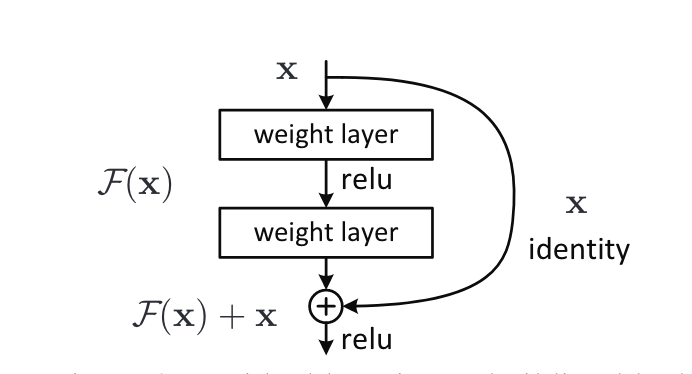
\includegraphics[width=0.6\textwidth]{figures/fig003.png}
    \caption{Aprendizado Residual: bloco}
    \label{fig:fig003}
\end{figure}

%--------------------------------------------------------
\section{Arquitetura Transformers}

A arquitetura \textit{Transformers} é uma estado da arte que se propôs a resolver as limitações das arquiteturas recorrentes e sua dificuldade em manter as relações entre pontos dentre as camadas recorrentes além das restrições vinculadas ao custo de computação sequencial. O modelo de arquitetura \textit{transformers} se utiliza do mecanismo de atenção e este se tornou parte integral de modelos de modelagem de sequências e transdução convincentes em várias tarefas, permitindo a modelagem de dependências sem considerar a distância entre elas nas sequências de entrada ou saída. Os \textit{transformers} como arquitetura descarta o uso de módulos de recorrência e se utiliza inteiramente do mecanismo de atenção para capturar as dependências globais entre entrada e saída. Os \textit{transformers} também são responsáveis por um ganho significante em paralelismo em sua execução \cite{vaswaniAttentionAllYou2023}.

\begin{figure}[htbp]
    \centering
    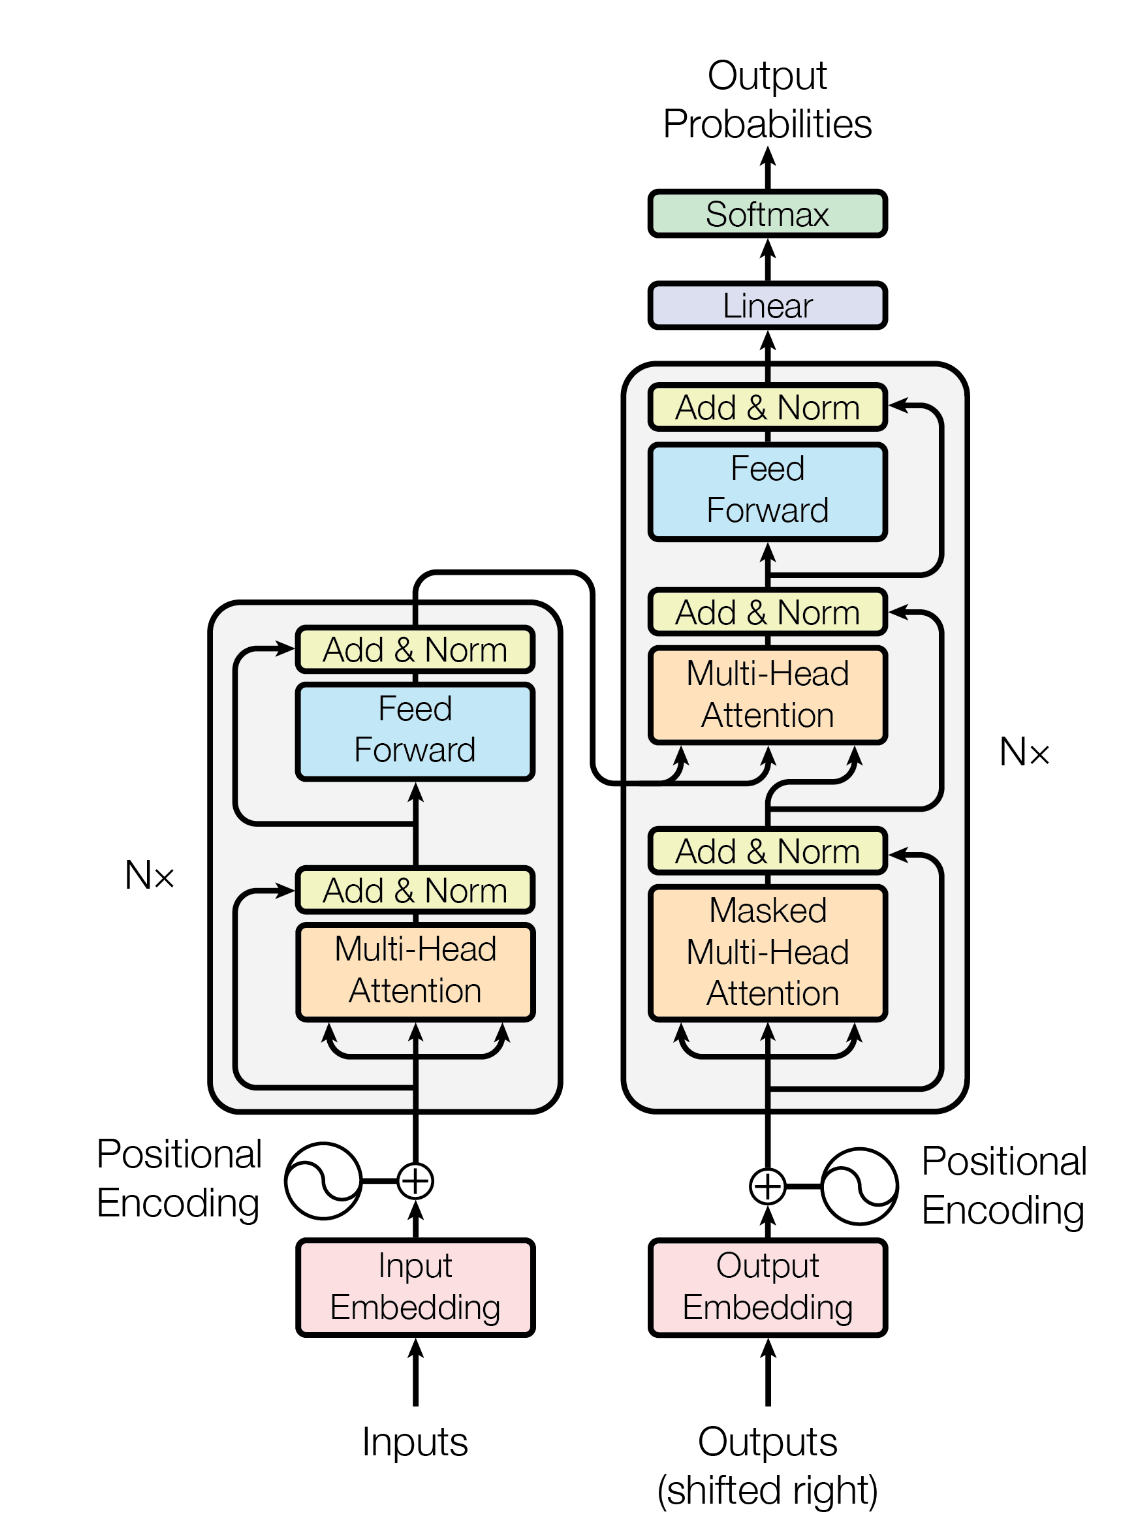
\includegraphics[width=0.6\textwidth]{figures/fig004.png}
    \caption{Arquitetura do \textit{Transformers}}
    \label{fig:fig004}
\end{figure}

O \textit{transformers} é composto por um \textit{Encoder} e um \textit{Decoder}, respectivamente o bloco da esquerda e direita \ref{fig:fig004}. Em ambos os \textit{Encoder} e \textit{Decoder}, tem-se como bloco cerne da rede o de atenção multi-cabeças. O mecanismo de atenção pode ser descrito mapeando uma \textit{query} e um par de chave e valor, onde a \textit{query}, chave e valor são todos vetores de saída. A saída é computada como uma soma ponderada dos valores onde o peso destinado a cada valor é computado por uma função de compatibilidade da query com a chave correspondente.

\begin{figure}[htbp]
    \centering
    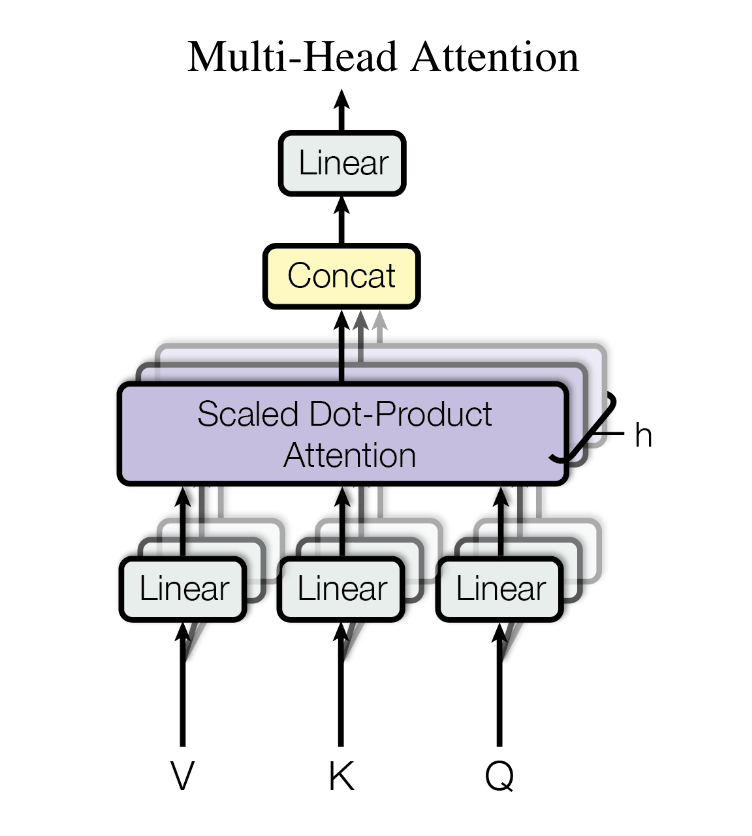
\includegraphics[width=0.6\textwidth]{figures/fig005.png}
    \caption{Arquitetura do \textit{Transformers}}
    \label{fig:fig005}
\end{figure}

O mecanismo de atenção é particularmente chamado de "Atenção de Produto Escalar Dimensionado" (Fig. \ref{fig:fig005}). A entrada consiste em consultas e chaves de dimensão $d_{k}$, e valores de dimensão $d_{v}$. É calculado os produtos escalares da consulta com todas as chaves e dividido cada um por $\sqrt{d_{k}}$. Em seguida, aplica-se uma função \textit{softmax} para obter os pesos sobre os valores. Na prática, é calculada a função de atenção em um conjunto de consultas simultaneamente, agrupadas em uma matriz $Q$. As chaves e os valores também são agrupados em matrizes $K$ e $V$. Calculamos a matriz de saídas como:

\begin{equation}
\text{Attention}(Q, K, V) = \text{softmax}\left(\frac{QK^T}{\sqrt{d_k}}\right)V
\label{eq:attention}
\end{equation}

Dos vários pontos de vantagem do mecanismo de atenção, pode-se citar: o total de poder computacional por camada, o total de computação que pode ser paralelizada e o já mencionado que seria relação de dependência entre dados que se encontram muito distantes um do outro, como também distâncias que necessitam ser percorridas frente e para trás na rede para identificar tais relações. Como benefício adicional, o mecanismo de atenção pode gerar modelos mais interpretáveis. Não apenas as cabeças de atenção individuais claramente aprendem a executar diferentes tarefas, muitas parecem exibir comportamentos relacionados à estrutura sintática e semântica das frases, no caso da aplicação em \textit{tokens} oriundos de textos.

%--------------------------------------------------------
\section{Considerações Finais do Capitulo}
\label{subsec:rcond_cap_3}

Os métodos de avaliação de cardiomiopatias, tanto via análise radiômicas por extração de textura quanto por aprendizado profundo obtiveram êxitos em análise de imagens médicas. Mesmo sabendo que estas técnicas de \textit{Machine Learning}, utilizando estes dados de textura podem ser insuficientes em capturar a complexidade e diversidade de informações a cerca do ventrículo como também pode ser afetada pela qualidade da imagem. Métodos pode aprendizado profundo podem aprender automaticamente semânticas de alto nível e informações representativas de imagens de RM sem necessidade de \textit{features} extraídas manualmente.
Métodos de aprendizado profundo tem obtido ótimos resultados em diagnósticos, segmentação, estadiamento e prognósticos. Todavia, o mesmo tem suas limitações como limitação dos dados, desafio geral na área médica, \textit{overfitting} e pouca interpretabilidade.

Dadas as vantagens e limitações discutidas, este trabalho tem como proposta a fusão de uma arquitetura de aprendizado profundo baseada no mecanismo de atenção que integras \textit{features} radiômicas e profundas para a identificação de cardiomiopatia. A arquitetura proposta é composta por: extração de \textit{features} radiômicas e profundas; redução de dimensionalidade para que ambas possuam tamanhos similares, redução estar utilizando \textit{F-Test}; concatenação das \textit{features}; aplicação do mecanismo de atenção e classificação binária do resultado. O esquemático pode ser conferido na Fig. \ref{fig:fig006}.

\begin{figure}[htbp]
    \centering
    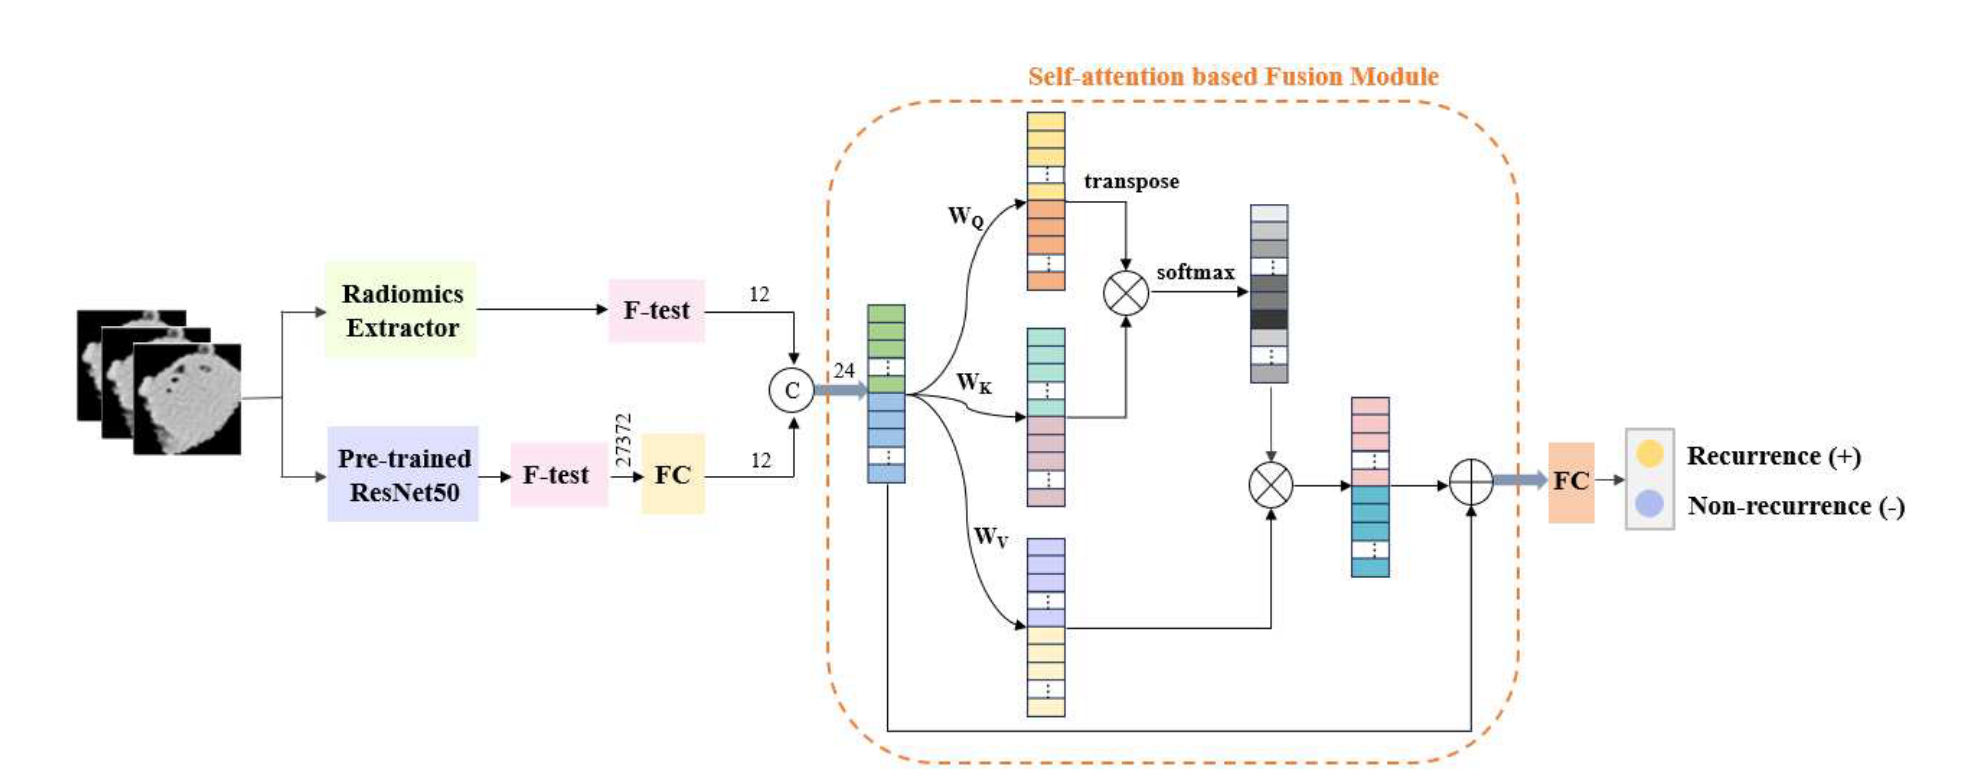
\includegraphics[width=1\textwidth]{figures/fig006.png}
    \caption{Arquitetura Proposta}
    \label{fig:fig00}
\end{figure}

Com esta abordagem, acredita-se que será aproveitada a riqueza de informações contidas nas imagens de RM e ajustadas de forma adaptativa a importância destas \textit{features}. A fusão das \textit{features} radiômicas manuais e as \textit{features} profundas, devem melhorar as habilidades de expressividade e generalização do modelo. Os resultados obtidos com testes iniciais no \textit{dataset} \textit{ACDC} demonstraram resultados promissores.

%--------------------------------------------------------
\section{Conjunto de Dados} \label{sec:conj_dados}

O conjunto de dados \textit{Automated Cardiac Diagnosis Challenge} (ACDC) foi criado a partir de exames clínicos reais adquiridos no hospital universitário de Dijon (França). Os dados adquiridos foram totalmente anonimizados e tratados de acordo com as regulamentações estabelecidas pelo comitê ético local do hospital de Dijon. O conjunto de dados cobre várias patologias bem definidas com casos suficientes para (1) treinar adequadamente métodos de aprendizado de máquina e (2) avaliar claramente as variações dos principais parâmetros fisiológicos obtidos a partir de cine-RM (em particular volume diastólico e fração de ejeção). O conjunto de dados é composto por 150 exames (todos de pacientes diferentes) divididos em 5 subgrupos distribuídos igualmente (4 patológicos mais 1 grupo de sujeitos saudáveis) conforme descrito abaixo. Além disso, cada paciente vem com as seguintes informações adicionais: peso, altura, bem como os instantes das fases diastólica e sistólica \cite{bernardDeepLearningTechniques2018a}.
\chapter{Trabalhos Relacionados} \label{chap:trab_relacionados}

% Neste capítulo serão apresentados trabalhos correlatos a este em ordem cronológica de
% publicação. Cada seção é referente a um tópico desta pesquisa, sendo as duas primeiras (Seções
% 3.1 e 3.2), segmentação e classificação, relacionadas a tarefas de visão computacional e divididas entre trabalhos envolvendo a criação de bases de dados (Seções 3.1.1 e 3.2.1) e de modelos
% (Seções 3.1.2 e 3.2.2) para cada um dos tópicos em questão. A Seção 3.3, reconhecimento automático de dor em recém-nascidos, traz algumas das abordagens criadas em função dos anos,
% para contextualização sobre as técnica disponíveis no meio.

Aplicar a unificação de técnicas radiômicas e \textit{deeplearning} em cardiomiopatias já são objeto de estudo em diversas pesquisas recentes.
Neste capítulo serão apresentados trabalhos e metodologias correlatos ao esforço de outros autores a cerca deste tema. As seções se referem a um tópico ou metodologia aplicados nesta pesquisa sendo a primeira (Seção \ref{sec:rev_sistematica}) responsável pela revisão sistemática da literatura.

%---------------------------------------------------------
\section{Revisão Sistemática da Literatura} \label{sec:rev_sistematica}

Para a fase exploratória dos trabalhos relacionados, foi utilizada a ferramenta \textit{Parsifal} com o objetivo de identificar estudos onde se aplica a análise radiômica no contexto de cardiopatia. O objetivo inicialmente definido foi o seguinte: "Identificar estudos onde se aplica análise radiômica a cardiopatia. Em segunda opção, alguma outra doença de natureza cardíaca". A pesquisa teve como objetivo responder as seguintes perguntas: quais desafios descritos nos estudos prévios e se há replicabilidade da proposta. As palavras chaves selecionadas são: \textit{cardiac}, \textit{cardiomyopathy} e \textit{radiomics}. A palavra de busca selecionada foi: ``\textit{radiomics} AND (\textit{cardiac} OR \textit{cardiomyopathy})'' com o intuito de filtrar os resultados de forma a identificar onde na ciência poderia identificar a interseção de ambas as abordagens(radiômica e \textit{deep}). Os resultado da busca pode ser conferido na Tabela \ref{tab:resultado_busca}. 

\begin{table}[hbtp]
    \centering
    \renewcommand{\arraystretch}{1.4} % default é 1 
    \begin{tabular}{|c|c|}
    \hline 
          \textbf{Origem} & \textbf{Artigos}  \\ 
    \hline 
        IEEE & 6 \\ 
        PUBMED & 19 \\ 
        Science@Direct & 24 \\ 
    \hline 
    \end{tabular} 
    \caption{Resultados dos Artigos}
    \label{tab:resultado_busca}
\end{table}

Em posse dos resultados, alguns critérios de aceitação foram aplicados como pode ser visto na Tabela \ref{tab:criterios}).

\begin{table}[hbtp]
    \centering
    \renewcommand{\arraystretch}{1.4} % default é 1 
    \begin{tabular}{|l|l|}
    \hline 
          \multicolumn{1}{|c|}{\textbf{Critério de Inclusão}} & \multicolumn{1}{c|}{\textbf{Critério de Exclusão}}  \\ 
    \hline 
        \quad Contém ressonância magnética? & \quad Estudos Duplicados   \\ 
        \quad O objeto de estudo é o coração? & \quad Estudos Secundários ou Terciários \\
        \quad Usa análise de textura? & \quad Estudos que não estão em PT ou EN\\
        \quad Utiliza análise radiômica? & \quad Leitura cinza  \\
        \quad É cardiomiopatia? & \quad Não aplica técnicas computacionais\\
        & \quad Não trata do coração \\
        & \quad Não usa RM \\
        & \quad Trabalho que atua somente com dados genômicos \\ 
    \hline 
    \end{tabular} 
    \caption{Critérios de Inclusão e Exclusão}
    \label{tab:criterios}
\end{table}

Critérios de aceitação também foram aplicados e podem ser conferidos na Tabela \ref{tab:questoes}. Dentre cada uma das seis perguntas, calculamos a nota usando como pontuação 1 para sim, 0,5 para parcial e 0 para talvez. Como nota de corte usamos o valor 3, ou seja, qualquer artigo que não alcance o valor mínimo de 3, é descartado. Uma vez aplicado os critérios de aceitação, restaram 18 artigos dos 49 artigos iniciais.

\begin{table}[hbtp]
    \centering
    \renewcommand{\arraystretch}{1.4} % default é 1 
    \begin{tabular}{|l|}
    \hline 
          \multicolumn{1}{|c|}{\textbf{Questões}} \\ 
    \hline 
        \quad É descrita as limitações do estudo? \\
        \quad Há um experimento bem descrito para avaliar a proposta? \\
        \quad Há mais de 2 autores? \\
        \quad O trabalho apresenta resultados? \\
        \quad A introdução apresenta o problema de forma clara \\
        \quad É análise sistemática da literatura? \\
    \hline 
    \end{tabular} 
    \caption{Questões de Aceitação}
    \label{tab:questoes}
\end{table}

%---------------------------------------------------------
\section{Análise Radiômica com Atenção}
\label{sec:analise_radiomica}

 \citeauthor{jiangMRIBasedRadiomics2021} \citeyear{jiangMRIBasedRadiomics2021} conduziram um estudo abrangente que aproveita as capacidades do aprendizado de máquina para melhorar os processos diagnósticos em oncologia, especificamente focando no câncer de colo de útero em estágio inicial. Sua pesquisa, intitulada "Abordagem Radiômica Baseada em Ressonância Magnética com Aprendizado Profundo para Predição de Invasão Vascular em Câncer de Colo de Útero em Estágio Inicial", foca na aplicação de técnicas de aprendizado profundo em dados de ressonância magnética multiparamétrica para prever a invasão vascular, um fator crítico para determinar a agressividade do câncer de colo de útero e informar estratégias de tratamento.

O estudo utilizou um conjunto substancial de dados compreendendo 1.070 imagens de ressonância magnética com contraste dinâmico T1 (DCE-T1) e 986 imagens de ressonância magnética ponderada em T2 (T2WI) coletadas de 167 pacientes diagnosticadas com câncer de colo de útero em estágio inicial entre janeiro de 2014 e agosto de 2018. Os pesquisadores empregaram uma nova estrutura de aprendizado profundo que integrou esses dois tipos distintos de varreduras em imagens RM para criar um modelo preditivo robusto. Implementando uma estratégia de aprendizado de conjunto com atenção, o modelo efetivamente distinguiu entre casos com invasão vascular e aqueles sem. Quatro modelos de CNN foram utilizados: VGGNet, GoogLeNet (Inception-v3), Residual Network (ResNet) e DenseNet. Um módulo padrão de squeeze-and-excitation (SE)  e o módulo de atenção de bloco convolucional (CBAM)  foram introduzidos após cada bloco de convolução da rede AdaptedVGG19 para fornecer um AdaptedVGG19-SE e um AdaptedVGG19-CBAM, respectivamente. A arquitetura proposta é vista na figura \ref{fig:fig007}.

O desempenho preditivo dos modelos foi rigorosamente avaliado usando a área sob a curva (ROC), com os modelos finais alcançando uma alta área sob a curva (AUC) de 0.911. Essa alta AUC indica uma forte capacidade do modelo para classificar corretamente a presença ou ausência de invasão vascular, com métricas de sensibilidade e especificidade também demonstrando precisão diagnóstica substancial.

Esta pesquisa demonstra o potencial de integrar algoritmos de aprendizado profundo com dados de imagem complexos para melhorar as avaliações diagnósticas pré-operatórias. Os achados de \citeauthor{jiangMRIBasedRadiomics2021} sugerem que tais abordagens analíticas avançadas podem fornecer suporte substancial na tomada de decisões clínicas, potencialmente levando a planos de tratamento mais personalizados e melhores resultados para os pacientes.

No contexto da pesquisa contínua em imagens médicas e diagnóstico de câncer, a metodologia e os resultados de \citeauthor{jiangMRIBasedRadiomics2021} fornecem um exemplo convincente do potencial da inteligência artificial para revolucionar os processos diagnósticos em oncologia. O uso de ressonância magnética multiparamétrica e modelos sofisticados de aprendizado de máquina exemplifica as abordagens inovadoras que estão sendo desenvolvidas para enfrentar os desafios da detecção precoce e precisa de câncer.

\begin{figure}[htbp]
    \centering
    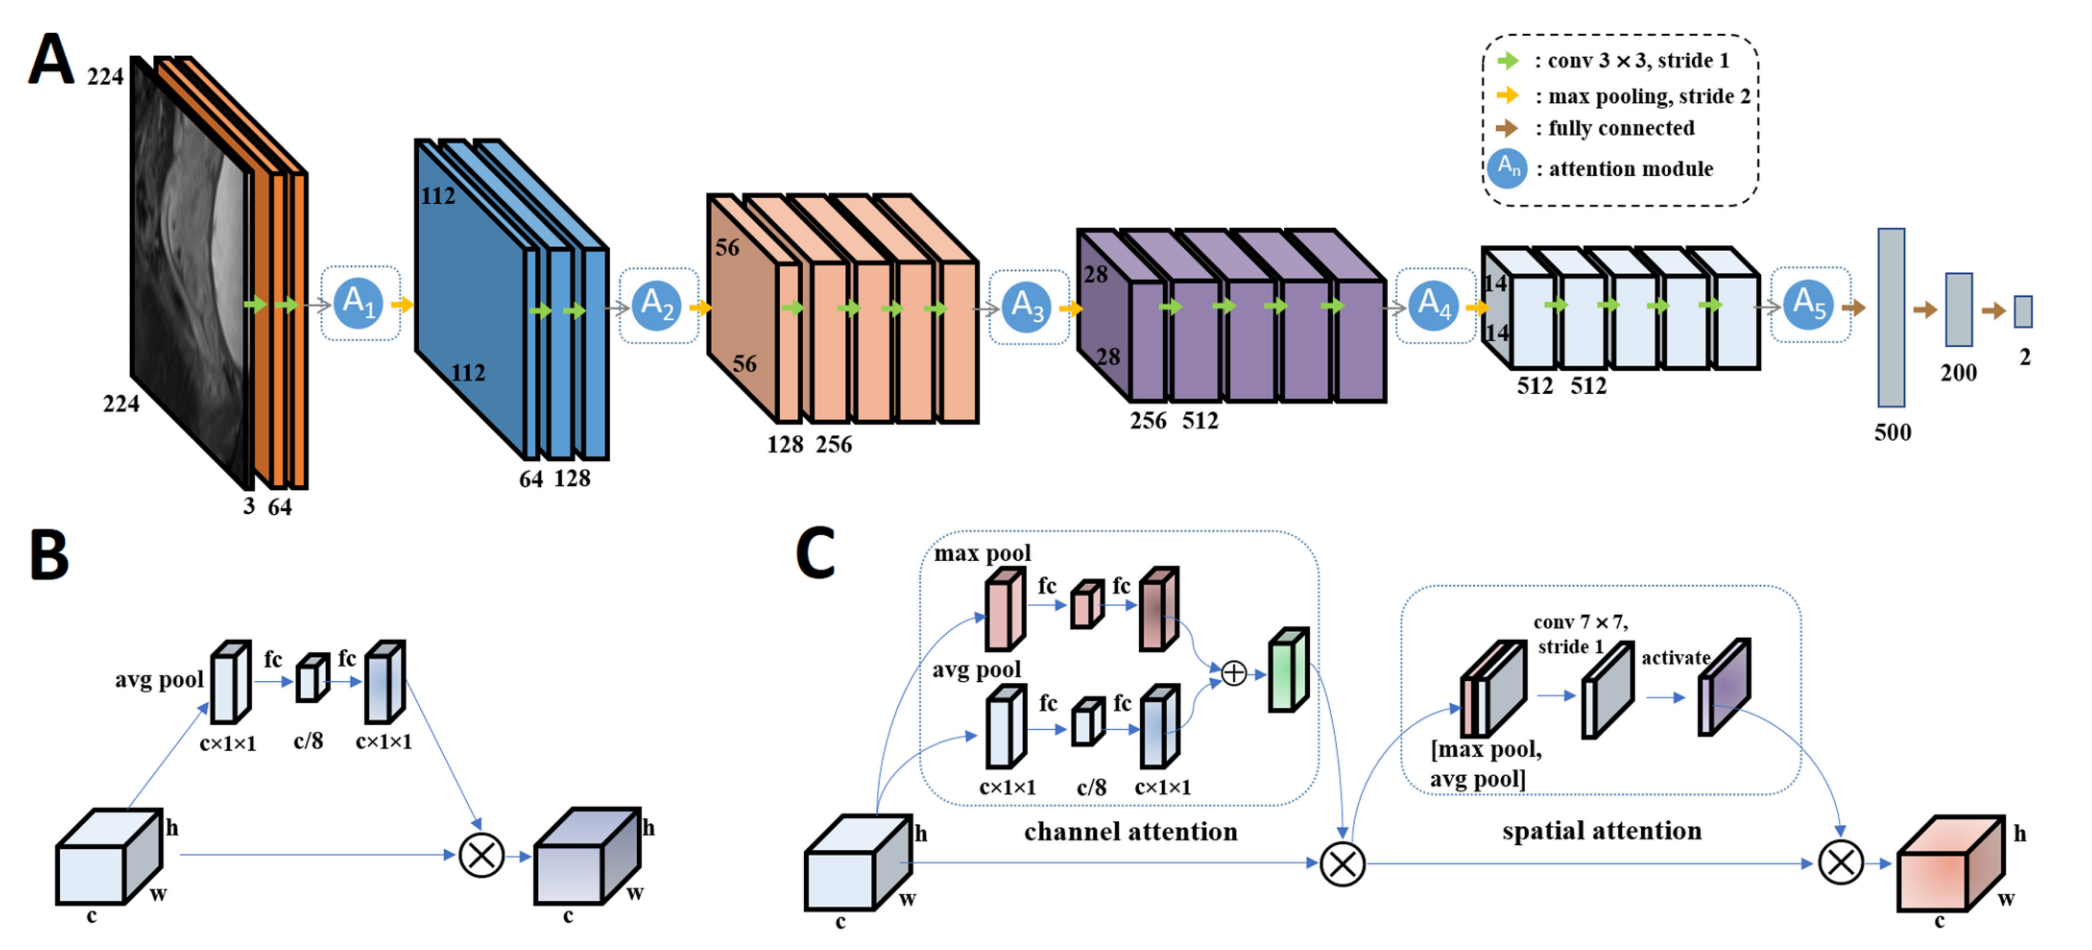
\includegraphics[width=0.8\textwidth]{figures/fig007.png}
    \caption{Fonte: \cite{jiangMRIBasedRadiomics2021}}
    \label{fig:fig007}
\end{figure}

%---------------------------------------------------------
Em outro trabalho, \cite{renBiLSTMMultiheadAttentionbased2023} desenvolveram um modelo avançado usando uma rede Bi-LSTM (memória de longo prazo bidirecional) combinada com um mecanismo de atenção de múltiplas cabeças, utilizando \textit{features} radiômicas e imagens TC de lesões, para aprimorar a diferenciação dos principais subtipos de adenocarcinoma pulmonar, integrando assinaturas radiômicas com características radiológicas de tomografias computadorizadas. O estudo recrutou 421 pacientes de três hospitais, confirmados com adenocarcinoma in situ, adenocarcinoma minimamente invasivo ou adenocarcinoma invasivo, com base na análise de 427 lesões.

A metodologia empregada envolveu a extração de assinaturas radiômicas usando o software `\textit{PyRadiomics}' das regiões de lesões identificadas em cada imagem de tomografia computadorizada. As 100 principais características foram então selecionadas através do método de classificação de características de máxima relevância e mínima redundância. Um modelo preditivo foi subsequentemente desenvolvido empregando essas características juntamente com características radiológicas, usando a estrutura Bi-LSTM e atenção múltipla para classificar as lesões.

O desempenho diagnóstico do modelo foi quantitativamente impressionante, alcançando valores da área sob a curva (AUC) de 0,985, 0,94 e 0,981 nos grupos de treinamento, teste e validação, respectivamente, com precisões correspondentes de 0,92, 0,976 e 0,91. Além disso, comparações foram feitas com dois outros modelos — rede neural convolucional (CNN) + atenção múltipla, e LSTM + atenção múltipla — demonstrando que o modelo Bi-LSTM e atenção múltipla superou essas alternativas em precisão e acurácia no conjunto de testes.

Esta pesquisa destaca a utilidade potente da combinação de técnicas avançadas de aprendizado de máquina com análises radiômicas e radiológicas detalhadas para refinar o processo diagnóstico para subtipos de adenocarcinoma pulmonar, potencialmente orientando abordagens de tratamento mais personalizadas baseadas na caracterização do subtipo.

%---------------------------------------------------------
 \cite{aiSelfAttentionBasedFusion2023} conduziram um estudo inovador intitulado ``Um Modelo de Fusão Baseado em Autoatenção de Características Radiômicas e Profundas para Previsão de Recorrência Precoce em CPNP'', que aborda o significativo desafio de prever a recorrência precoce em câncer de pulmão de células não pequenas usando técnicas avançadas de aprendizado de máquina. Sua pesquisa aproveita o mecanismo de autoatenção para fundir características radiômicas manuais e características de aprendizado profundo extraídas de imagens de TC, com o objetivo de aumentar a precisão preditiva e robustez para recorrência precoce em câncer de pulmão de células não pequenas.

O estudo começou empregando diversas técnicas de aprendizado de máquina para extrair uma variedade de características artesanais de imagens de TC, incluindo atributos de textura, forma e escala de cinza. Para capturar informações semânticas de alto nível e de representação, uma rede ResNet50 pré-treinada foi utilizada para a extração de \textit{features} profundas. Essas características extraídas foram então fundidas com um vetor de características extraído de dados de texturas de imagens radiômicas e unificado usando um módulo de fusão de autoatenção inovador desenvolvido pelos pesquisadores. Este módulo otimiza e pondera o vetor de características fundidas, aproveitando plenamente o mecanismo de autoatenção para melhorar as capacidades de previsão do modelo. A arquitetura pode ser conferida na Figura \ref{fig:fig008}.

Os resultados experimentais, avaliados no conjunto de dados público Cancer Imaging Archive (TCIA), demonstraram que o modelo proposto superou significativamente os métodos existentes na previsão de recorrência precoce. O modelo exibiu melhorias substanciais em precisão de classificação, sensibilidade, especificidade e a área sob a curva (AUC), destacando seu potencial para guiar o tratamento em estágio inicial e melhorar as taxas de sobrevivência para pacientes com câncer de pulmão de células não pequenas.

Este estudo exemplifica a aplicação de técnicas avançadas de aprendizado de máquina em imagens médicas e oncologia, fornecendo um método robusto para a previsão de recorrência precoce que poderia impactar significativamente os resultados clínicos e as estratégias de tratamento em câncer de pulmão.

\begin{figure}[htbp]
    \centering
    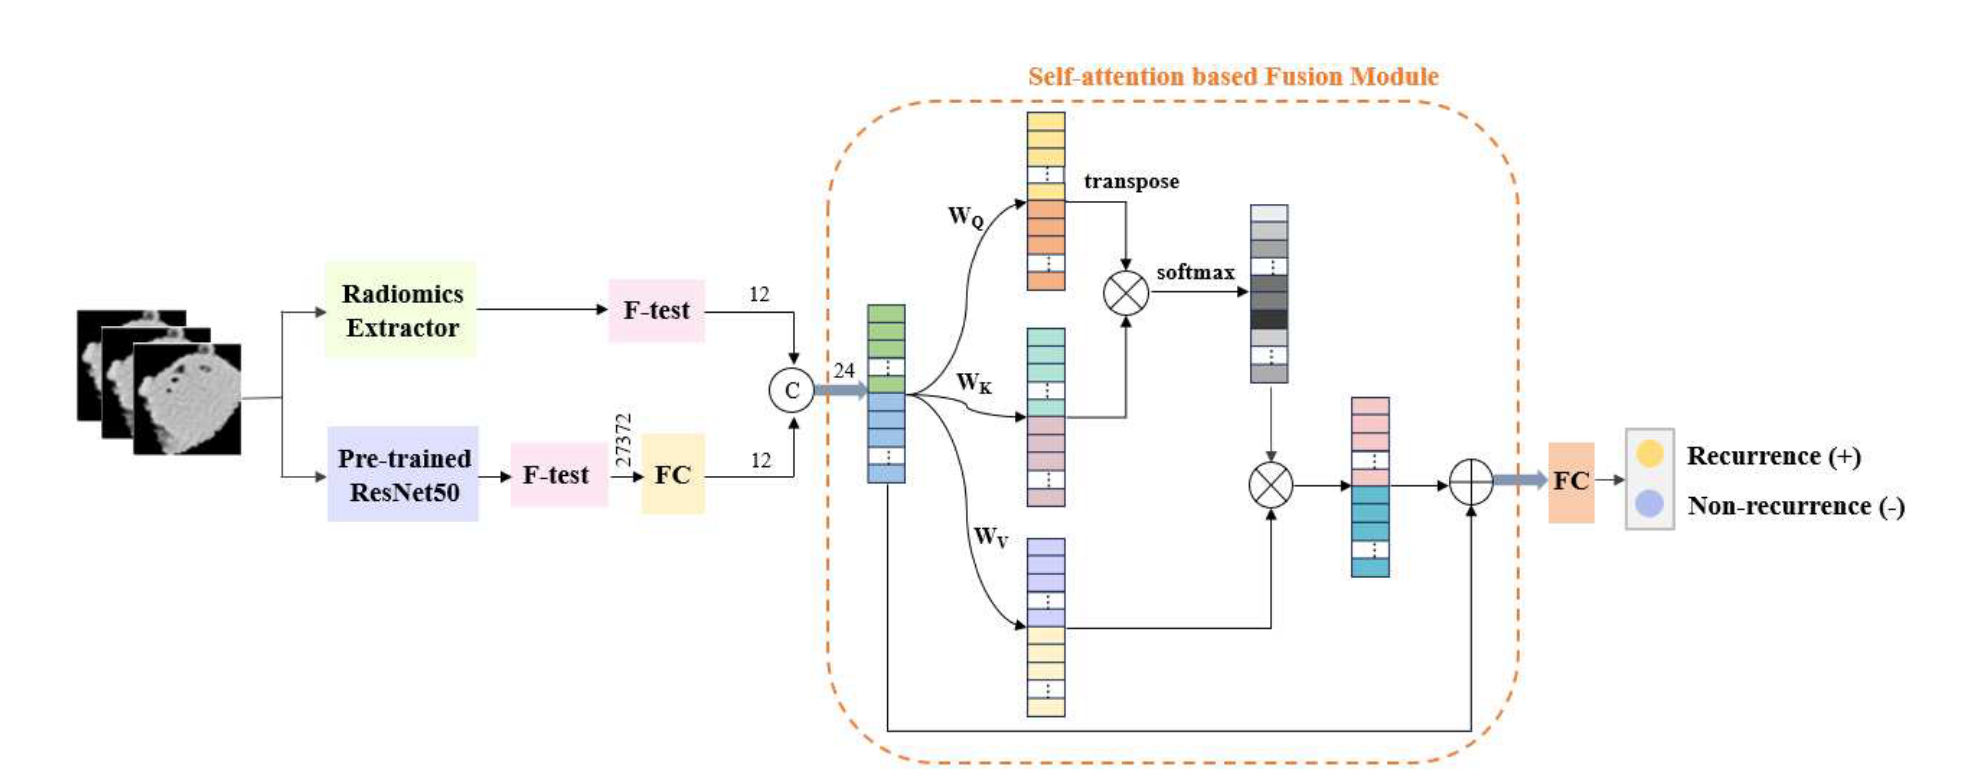
\includegraphics[width=1\textwidth]{figures/fig008.png}
    \caption{Fonte: \cite{aiSelfAttentionBasedFusion2023}}
    \label{fig:fig008}
\end{figure}
%---------------------------------------------------------

\cite{iranmehrImprovedPredictionMGMT2022} desenvolveram uma rede de aprendizado profundo inovadora que utiliza um mecanismo baseado em atenção para aprimorar a previsão do estado de metilação do gene MGMT em glioblastoma muiltifoma (GBM), o tipo mais agressivo de tumor cerebral. Pacientes com GBM possuem uma expectativa muito baixa, entre 18 e 24 meses e requerem tratamentos agressivos, como por exemplo, quimioterapia. Sua pesquisa, apresentada em "Improved Prediction of MGMT Methylation Status in Glioblastoma using a Deep Attention Network", destaca um avanço significativo nas capacidades diagnósticas não invasivas para GBM, que tipicamente tem uma taxa de sobrevivência de apenas 18 meses.

O estudo foca no gene MGMT, cujo estado de metilação é crucial para determinar a eficácia da quimioterapia em pacientes com GBM. As análises radiômicas tradicionais, embora úteis, muitas vezes não capturam os recursos intrincados necessários para uma previsão precisa da metilação. \citeauthor{iranmehrImprovedPredictionMGMT2022} propõem um modelo que integra características radiômicas manuais com técnicas de aprendizado profundo, melhorando a extração de características e a precisão da previsão de GBM.

O modelo introduzido pela equipe utiliza uma combinação de mecanismos de atenção \textit{squeeze} e sequencial para priorizar fatias e regiões relevantes dentro das imagens de ressonância magnética, respectivamente. Esse método não apenas melhora o foco em áreas significativas, mas também aprimora a interpretabilidade geral do modelo. O modelo proposto (Fig. \ref{fig:fig009}) consiste de três etapas: 1) Um modelo base para extrair as \textit{features}, 2) uma rede de atenção temporal e espacial e 3) uma rede de classificação para prever se o exame é metilado ou não metilado. 

\begin{figure}[htbp]
    \centering
    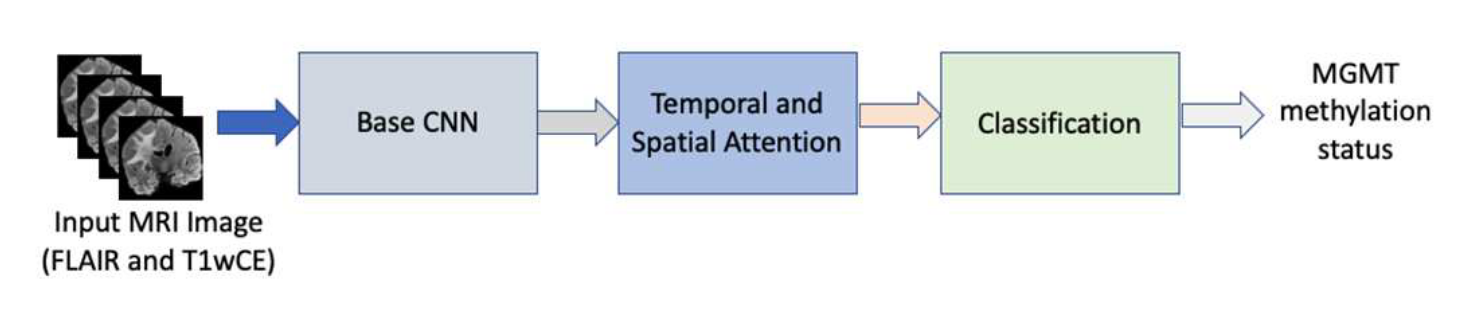
\includegraphics[width=1\textwidth]{figures/fig009.png}
    \caption{Método proposto. \textit{Densenet} foi utilizado como modelo base. A saída da rede densa é alimentada pela rede de atenção que pode priorizar as fatias e regiões. A saída da rede de atenção é enviada à rede de classificação binária para prever o status de metilação do MGMT.}
    \label{fig:fig009}
\end{figure}

O modelo base consiste em uma \textit{DenseNet}. Segundo o autor, a \textit{Densenet} pode suportar milhares de camadas e ser resistente ao \textit{overfitting}. A saída da rede densa é fornecida para a rede de \textit{squeeze} e \textit{self attention} conforme mostrado na Fig. \ref{fig:fig010}. Cada exame consiste em várias fatias e a \textit{squeeze attention} priorizará as fatias, usando o agrupamento médio global seguido por duas camadas densas separadas e depois o produto escalar com a entrada inicial. A saída da \textit{squeeze attention} é fornecida à rede de \textit{self attention}. Após a aplicação da \textit{self attention}, o mapa de atenção contém pixels com uma seção de maior importância em cada fatia. Com a rede de \textit{self attention}, é possível enfatizar pixels e regiões de diferentes independente da distância em que estes \textit{pixels} se localizam pela imagem. Múltiplas regiões com diferentes tamanhos geradas a partir de regiões integrais são então fornecidas à \textit{attention} sequencial (SA). A rede SA adapta uma rede \textit{long short term memory} (LSTM), que é capaz de aprender dependências de longo prazo. A saída passa por uma camada densa e uma sigmoide para fazer a classificação.

Avaliado em várias métricas de classificação binária, o modelo alcançou a melhor área sob a curva (AUC) de 70,59, demonstrando sua superioridade em relação aos métodos existentes. Este trabalho fornece uma abordagem robusta e automática para capturar características críticas de imagens de ressonância magnética, avançando significativamente na previsão do estado de metilação em GBM em comparação com métodos anteriores. As implicações de tais avanços são profundas, potencialmente melhorando o planejamento de tratamentos personalizados e, em última análise, os resultados para os pacientes com glioblastoma.

\begin{figure}[htbp]
    \centering
    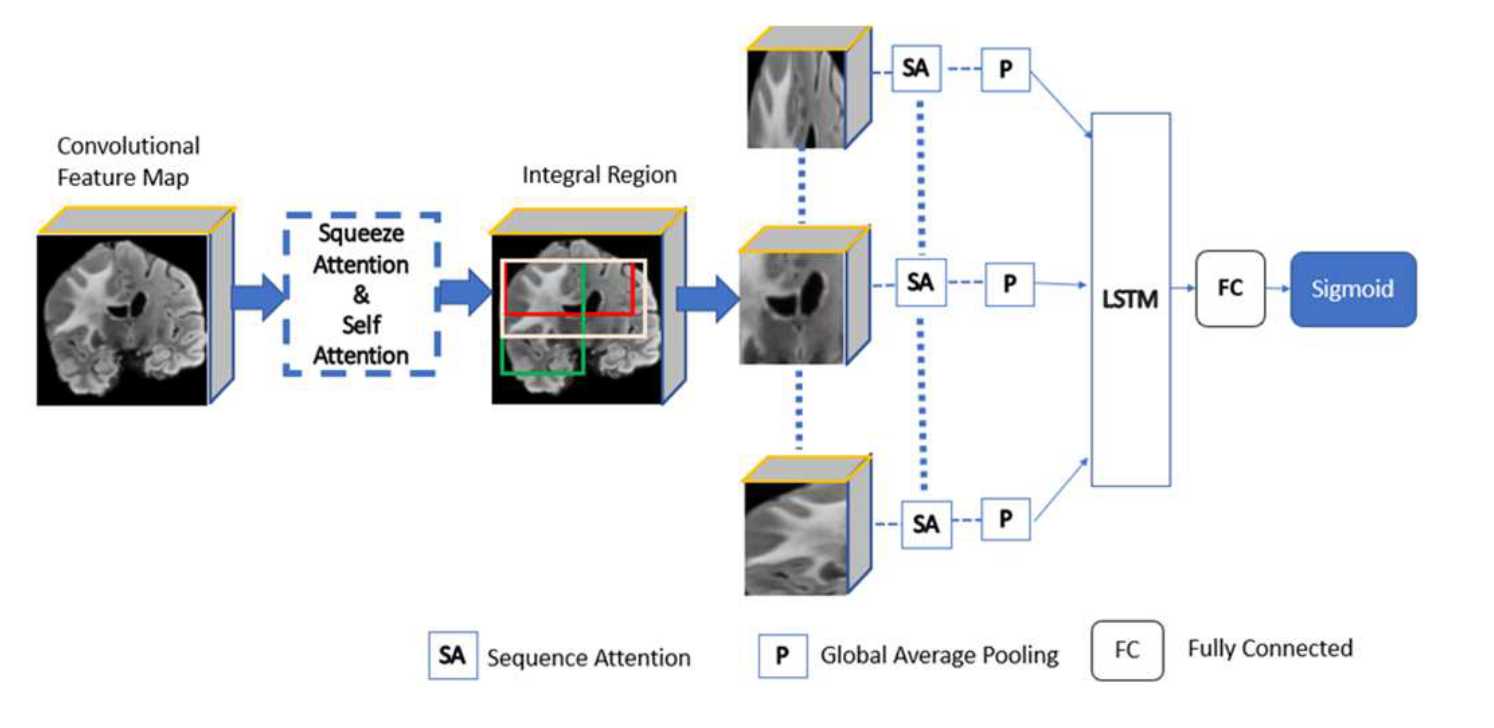
\includegraphics[width=1\textwidth]{figures/fig010.png}
    \caption{Fonte: \cite{iranmehrImprovedPredictionMGMT2022}}
    \label{fig:fig010}
\end{figure}

%---------------------------------------------------------
% \section{Considerações Finais do Capítulo}
% \label{sec:rcond_cap_3}
% \lipsum[2-4]
\chapter{Metodologia} 
\label{chap:metodologia}

O objetivo deste trabalho é propor e investigar uma arquitetura de aprendizado profundo que unifica \textit{features} de radiômica e \textit{features} profundas. Inicialmente, é empregado diversas técnicas de aprendizado de máquina para extrair \textit{features} manuais de imagens de RM, abrangendo textura, forma, escala de cinza, etc. Posteriormente, uma rede \textit{ResNet50} pré-treinada é utilizada para extrair \textit{features} profundas que encapsulam informações semânticas de alto nível e de representação das imagens de RM. Estas \textit{features} são então fundidas em um vetor de \textit{features} unificado. Para aprimorar a acurácia e a robustez, um módulo de \textit{self attention} foi desenvolvido. Utilizando o mecanismo de \textit{self attention}, este módulo otimiza e pondera o vetor de \textit{features} fundidas de forma eficaz.

%---------------------------------------------------------
\section{Conjunto de Dados}
As bases de imagens utilizadas neste trabalho não possuem acesso público. O acesso
a base ocorreu pela parceria existente entre o Centro Universitário FEI e o Instituto do Coração do Hospital das Clínicas da FMUSP (InCor).

%---------------------------------------------------------
\section{Métodos}
\label{sec:cap4_metodos}

%---------------------------------------------------------
\subsection{Features Radiômicas}
\label{subsec:cap4_features_radiomicas}

Foi extraído 72 \textit{features} radiômicas de fase diastólica, representada por um conjunto de fatias variando entre 6 e 18 \textit{frames}, de cada paciente usando matriz de coocorrência de níveis de cinza (GLCM) e estatísticas baseadas em histograma. Foi aplicado o filtro \textit{Laplace of Gaussian} (LoG) com cinco diferentes valores em cada parte para suavizar as imagens e realçar as bordas. Foi calculado \textit{features} GLCM como contraste, entropia, correlação, homogeneidade e energia para cada filtro LoG. Também é calculado \textit{features} de intensidade como média, variância, média dos percentis (10 e 90), desvio robusto da média absoluta, curtose e assimetria usando estatísticas de primeira ordem. Foram obtidos 78 \textit{features} radiômicas para cada paciente dentro da quantidade de fatias extraídas na fase diastólica.

%---------------------------------------------------------
\subsection{Unificando as Features}
\label{subsec:cap4_unificando_features}

Um vez em posse das features radiômicas, é aplicado um F-Test e reduz-se cada um dos vetores à 64 \textit{features}. Unificando ambos os vetores obtemos um vetor de \textit{features} de tamanho 128 o qual passará pelo mecanismo de \textit{attention}.

%---------------------------------------------------------
\section{Considerações Finais do Capítulo}
\label{sec:cap4_consideracoes_finais}

\lipsum[1-4]
\chapter{Proposta Experimental}
\label{chap:proposta}
\lipsum[2-4]

\section{Cronograma}
\label{sec:cronograma}

\lipsum[2-4]




\chapter{Resultados  Preliminares}
\label{chap:resultados_discussao}

\lipsum[2-4]

\chapter{Conclusão}
\label{chap:conclusao}

Esta dissertação tem como objetivo a utilização de descritor fractal em sistema de CBIR e também busca analisar o seu desempenho na recuperação de imagens de línguas similares a aquelas utilizadas como a “Imagem Pesquisa”. Durante o desenvolvimento do trabalho de pesquisa, foi possível validar que o descritor fractal possui um desempenho melhor quando comparado com outras técnicas para a encontrar a dimensão fractal de um objeto  e por conta disto, descriminam melhor a imagem, o que facilita a recuperação ou retorno de imagem similares em um banco de imagens.

Afim de validar a pesquisa, foi desenvolvido um modelo experimental para que seja eficiente em medir o desempenho do sistema de CBIR em recuperar imagens de línguas quando compradas com imagens de línguas com diagnóstico positivo para HAS, realizado conforme a metodologia e comprovação de profissionais especializados em MTC. Para avaliar o modelo foram promovidos testes preliminares e relatados nesta dissertação.

No atual estágio desta dissertação, o banco de imagens não está completo e aguarda as imagens das línguas com HAS positivo. Por isso os testes são preliminares e insuficientes para uma conclusão. No entanto, estes testes apontam que o sistema de CBIR possui uma Precisão de 98,95\% sendo que 85,26\% das imagens recuperadas está na primeira opção. Os testes preliminares também contemplaram a recuperação de línguas com fissuras, sendo o melhor resultado da AUC de 65,5\% e a recuperação de imagem conforme a sua cor, cujo resultado da AUC é de 71\%.

Esta dissertação utiliza o método \textit{boxcounting} para determinar a dimensão fractal das imagens e para isso foi utilizado a biblioteca Python PoreSpy que demonstra ser eficiente para encontrar o vetor de característica da imagem. Além disso, esta biblioteca permite que seja redefinido o vetor de característica permitindo configurar a quantidade de elementos para compô-lo. 

Este é um fato importante, porque os testes preliminares indicam a necessidade de ajustes no sistema de CBIR que pode ser melhorado adicionando mais variáveis da curva log-log ao vetor de características, o que é possível com a biblioteca Python PoreSpy.

A respeito das medidas de similaridade, o resultado dos testes preliminares demonstram que estão muito próximos e podem orientar que há equilíbrio entre os métodos utilizados para encontrar o resultado do cálculo da distância.

O banco de imagens é único e estará composto por duas bases de imagens de línguas que são distintas, sendo a primeira composta por pacientes Brasileiros, portanto, pessoas do ocidente com imagens de língua que não são homogêneas, ou seja, diferentes raças, idade e gêneros e que contempla o padrão ouro. O segundo banco é composto por 95 imagens de pacientes orientais, idosos e dos gêneros masculino e feminino. Todos os testes preliminares foram realizados exclusivamente com o segundo banco de imagens









\printbibliography
%\printindex

%\begin{anexo}

\appendix \centering \textbf{ANEXO 1} 


%\includepdf[pages=1-12]{documentos/ane1}

\appendix \centering \textbf{ANEXO 2}
%\includepdf [pages=1-7]{documentos/ane2}


%\end{anexo}





\end{document}
